% Chapter Template

\chapter{Hardware, Technologies, Toolchain and Programming Languages} % Main chapter title

\label{Hardware, Technologies, Toolchain and Programming Languages} % Change X to a consecutive number; for referencing this chapter elsewhere, use \ref{ChapterX}

%----------------------------------------------------------------------------------------
%	Hardware
%----------------------------------------------------------------------------------------

\section{Hardware}

%-----------------------------------
%	SUBSECTION 1
%-----------------------------------
\subsection{Xiaomi Mi Band}

The Xiaomi Mi Band\footnote{\href{http://www.mi.com/en/miband/}{\texttt{http://www.mi.com/en/miband/}}} (Figure \ref{fig:smartband}) is a wearable fitness tracker produced by Xiaomi. Xiaomi Mi Band was unveiled during a Xiaomi launch event on 22 July 2014.
\begin{figure}[h]
	\centering
	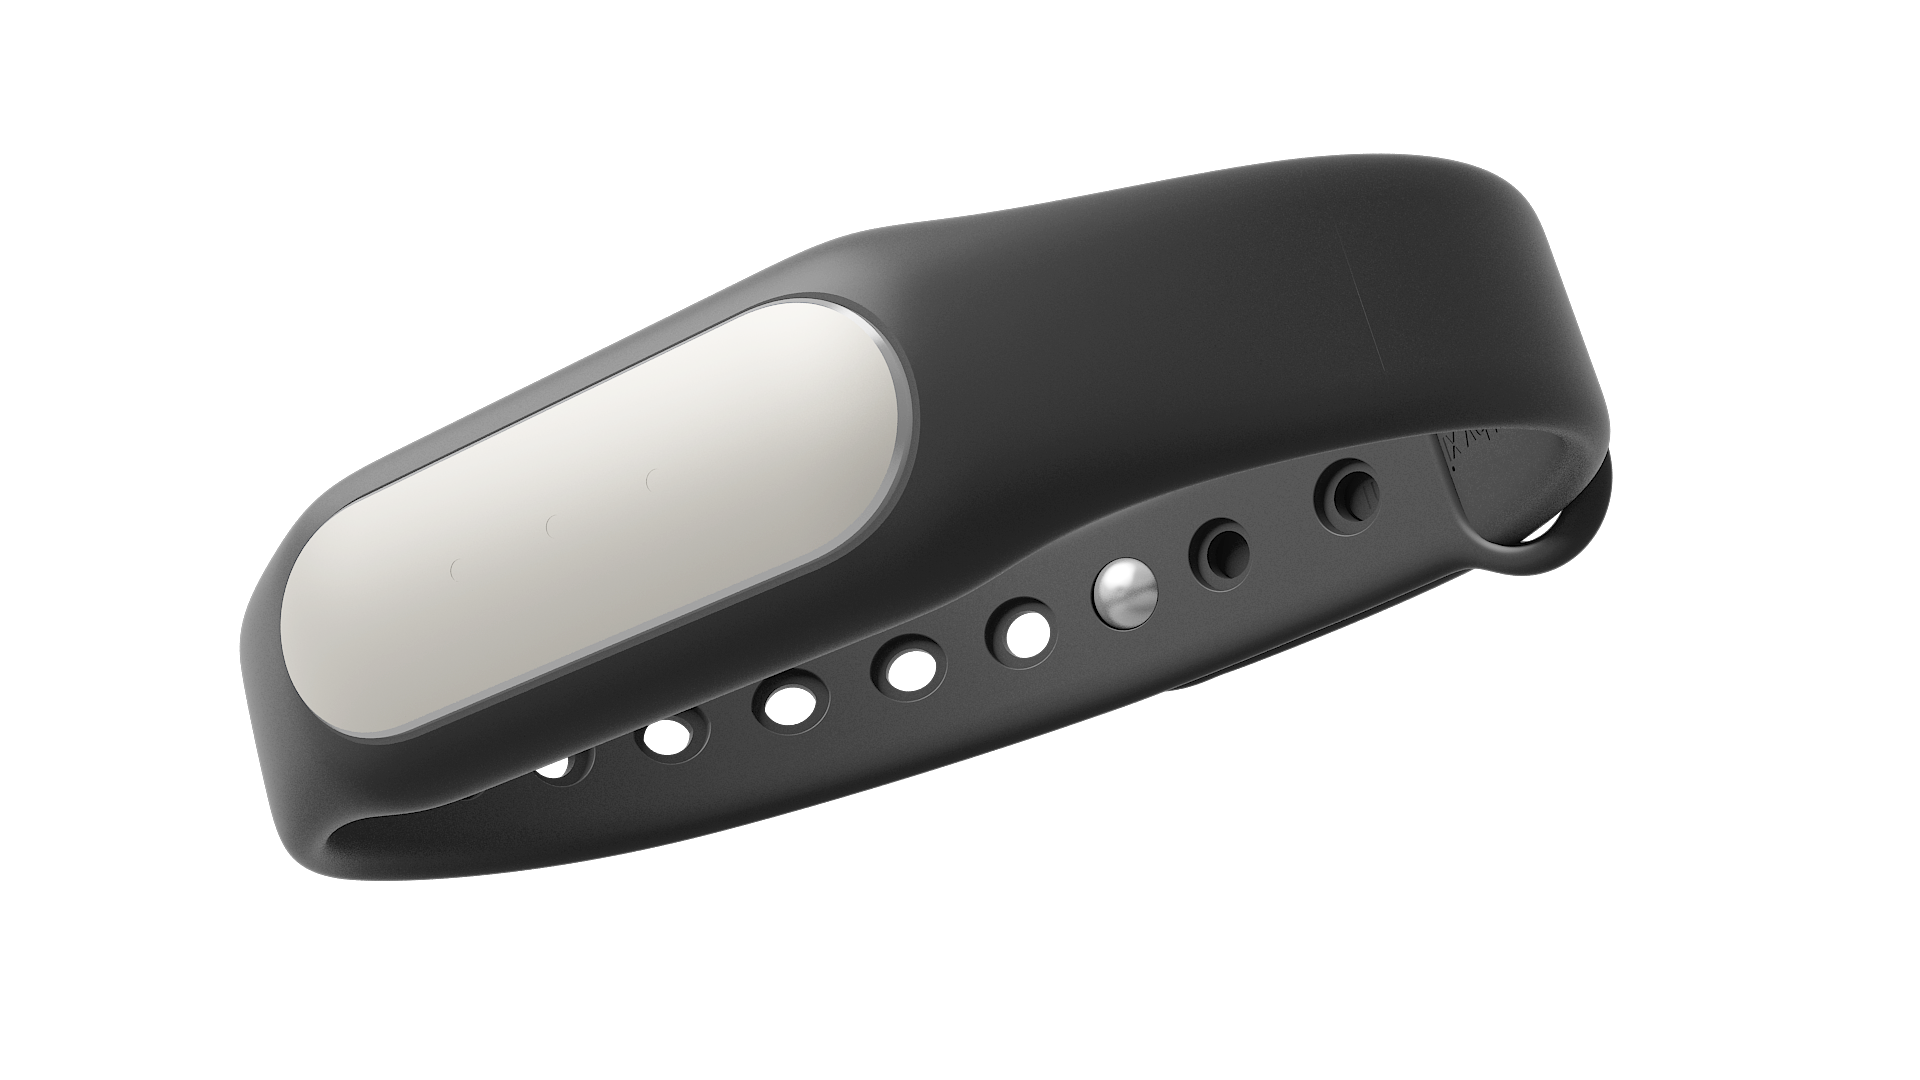
\includegraphics[width=0.7\linewidth]{images/smartband}
	\caption{Xiaomi Mi Band}
	\label{fig:smartband}
\end{figure}

Specifications:
\begin{itemize}
	\item Fitness monitor \& sleep tracker
	\item Sleep-cycle smart alarm
	\item Unlock your Android without a password
	\item 30-day standby power
	\item Water resistant (IP67)
	\item vibrate alert(call \& notification)
\end{itemize}

%-----------------------------------
%	SUBSECTION 2
%-----------------------------------
\subsection{Raspberry Pi}

The Raspberry Pi\footnote{\href{https://www.raspberrypi.org/help/what-is-a-raspberry-pi/}{\texttt{https://www.raspberrypi.org/help/what-is-a-raspberry-pi/}}} (Figure \ref{fig:raspberry})  is a series of small single-board computers developed in the United Kingdom by the Raspberry Pi Foundation to promote the teaching of basic computer science in schools and in developing countries. The original model became far more popular than anticipated, selling outside of its target market for uses such as robotics. Peripherals (including keyboards, mice and cases) are not included with the Raspberry Pi. Some accessories however have been included in several official and unofficial bundles.
\begin{figure}[h]
	\centering
	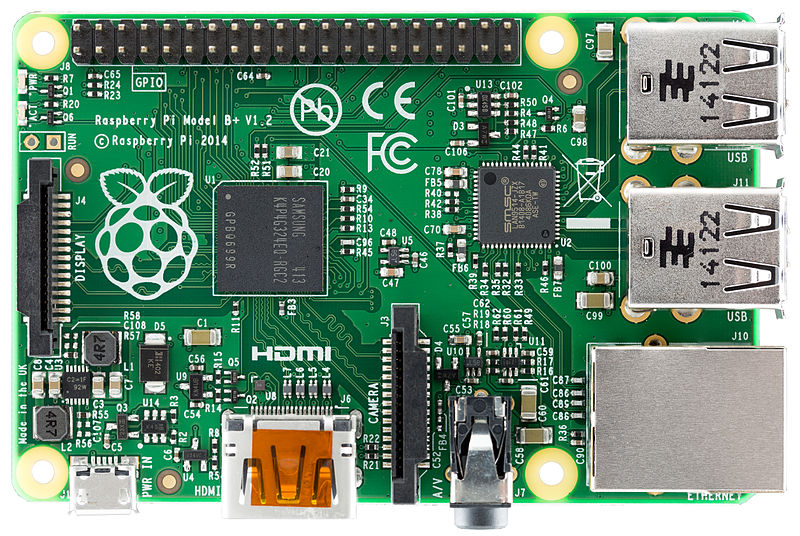
\includegraphics[width=0.5\linewidth]{images/raspberrypi.jpg}
	\caption{Raspberry Pi 1 model B+}
	\label{fig:raspberry}
\end{figure}

%----------------------------------------------------------------------------------------
%	Hardware, Technologies, Toolchain and Programming Languages
%----------------------------------------------------------------------------------------
\section{Toolchain}
In software, a toolchain is a set of programming tools that are used to perform a complex software development task or to create a software product, which is typically another computer program or a set of related programs. In general, the tools forming a toolchain are executed consecutively so the output or resulting environment state of each tool becomes the input or starting environment for the next one, but the term is also used when referring to a set of related tools that are not necessarily executed consecutively.

\section{Technologies and Programming Languages}

The software has three parts the backend, the frontend and the gateway, communicate with each other trow a RESTapi. So i will present the separately.

\subsection{Backend}

The backend is a java application the main framework is Spring Boot.

\subsection{Frontend}

\subsection{Gateway}